
\documentclass[]{article}
\usepackage{float}
\usepackage{rotating}
\usepackage[textwidth=170mm,bottom=20mm,top=25mm,headsep=8mm]{geometry}
\usepackage[utf8]{inputenc}
\usepackage[german]{babel}
\usepackage[T1]{fontenc}
\usepackage{graphicx}
\usepackage{amsmath}
\usepackage{amssymb}
\usepackage{amsfonts}
\usepackage{mathrsfs}
\usepackage{commath}
\usepackage{mathtools}
\usepackage{siunitx}
\usepackage{subcaption} %subfigures
\usepackage{textcomp}
\usepackage{xfrac}
\usepackage[section]{placeins}

\renewcommand\vec{\mathbf}
\DeclareMathOperator{\dift}{d^3 \!}
\newcommand*\chem[1]{\ensuremath{\mathrm{#1}}}
%%text über bilder
\usepackage[percent]{overpic}

\newcommand{\quadimage}[1]{
	\begin{overpic}#1
		\put (0,100)  {\bf \small (a)}
		\put (50,100) {\bf \small (b)}
		\put (0,50)   {\bf \small (c)}
		\put (50,50)  {\bf \small (d)}
	\end{overpic}
}
\newcommand{\reconimage}[1]{
	\begin{overpic}#1
		\put (0,100)  {Original}
		\put (50,100) {IPR}
		\put (0,50)   {Wiener}
		\put (50,50)  {Holo}
	\end{overpic}
}

\begin{document}
\section{Theorie Simulation}
\paragraph{MSFT}
\begin{equation}
	\phi\propto\int \delta\eta(\vec{r}) e^{-i\vec{q}\cdot \vec{r}} \dif \vec{r} \, .
\end{equation}
\begin{align}
	k^2=(k-q_\parallel)^2+q_{\perp}^2                  
	\Leftrightarrow q_\parallel=k-\sqrt{k^2-q_\perp^2} \,.
\end{align}
\begin{equation}
	\label{eq:msft}
	\phi\approx\sum_n{\mathscr{F}\left[\delta\eta\right] e^{-in\delta_z\left(k-\sqrt{k^2-q_\perp^2}\right) }} \, .
\end{equation}

\paragraph{Multislice Propagation}
\begin{equation}
	\bar{\phi}\left(q_x,q_y,z+\Delta z\right)=\bar{\phi}(z)e^{i\Delta z\sqrt{k^2-(q_x+q_y)^2}} \, ,
\end{equation}

\begin{equation}
	\phi(x,y,z+\Delta z)=\phi e^{i\delta n\left(z\right) \Delta z} \, .
\end{equation}

\begin{figure}
	\centering
	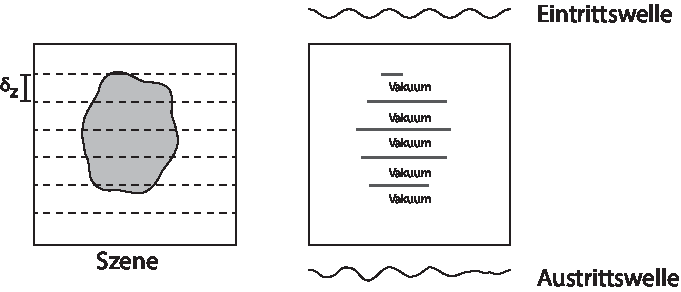
\includegraphics[width=0.9\textwidth]{images/multislice.pdf}
	\caption[Prinzip Multislice Propagation]{Prinzip Multislice Propagation: Die Szene wird in einzelne Schichten zerlegt und die Wechselwirkung mit der Materie jeder einzelnen Schicht in auf eine in dieser Schicht liegenden Ebene reduziert. Zwischen diesen Ebenen wird eine Vakuumpropagation angewendet.}
	\label{fig:multislice}
\end{figure} 

\paragraph{Thibault}

\begin{equation}
	\bar{\Phi}(z)=\bar{G}\ast_z\left[\bar{\delta\eta}\ast_{q_\perp} \bar{\Phi}\right]
\end{equation}
mit
\begin{equation}
	\bar{G}=\frac{1}{2\pi}\frac{ik^2}{\sqrt{k^2-q_\perp^2}}e^{iz(\kappa-k)}
\end{equation}
Faltungsintegral aufspalten:
\begin{equation}
	\bar{\Phi}(z+\Delta z)=
	\int_{\Delta z}^{\infty} \bar{G}(z')\left[\bar{\delta\eta}\ast_{q_\perp} \bar{\Phi}\right](z+\Delta z-z')\dif z'
	+
	\int_{0}^{\Delta z} \bar{G}(z')\left[\bar{\delta\eta}\ast_{q_\perp} \bar{\Phi}\right](z+\Delta z-z')\dif z'
\end{equation}
1. Summand: Substitution ($z'\rightarrow z''+\Delta z$)
\begin{align*}
	  & \stackrel{\hphantom{z'\rightarrow z''+\Delta z}}{\hphantom{=}} 
	\int_{\Delta z}^{\infty} \bar{G}(z')\left[\bar{\delta\eta}\ast_{q_\perp} \bar{\Phi}\right](z+\Delta z-z')\dif z'\\
	  & \stackrel{z'\rightarrow z''+\Delta z}{=}                       
	\int_{0}^{\infty} \bar{G}(z''+\Delta z)\left[\bar{\delta\eta}\ast_{q_\perp} \bar{\Phi}\right](z-z'')\dif z''\\
	  & \stackrel{\hphantom{z'\rightarrow z''+\Delta z}}{=}            
	e^{i\Delta z(\kappa-k)}\int_{0}^{\infty} \frac{1}{2\pi}\frac{ik^2}{\sqrt{k^2-q^2_\perp}}e^{iz''(\kappa-k)}\left[\bar{\delta\eta}\ast_{q_\perp} \bar{\Phi}\right](z-z'')\dif z''\\
	  & \stackrel{\hphantom{z'\rightarrow z''+\Delta z}}{=}            
	e^{i\Delta z(\kappa-k)}\bar{\Phi}(z)  \,,
\end{align*}
2. Summand:Rieman-Obersumme mit einem einzigen Stützpunkt bei $\Delta z$  ( Fehler von der Ordnung $\Delta z$):
\begin{equation}
	\int_{0}^{\Delta z} \bar{G}(z')\left[\bar{\delta\eta}\ast_{q_\perp} \bar{\Phi}\right](z+\Delta z-z')\dif z'
	\approx
	\Delta z \bar{G}(\Delta z)\left[\bar{\delta\eta}\ast_{q_\perp} \bar{\Phi}\right](z)
\end{equation}
Näherung für die Welle bei $z+\Delta z$:
\begin{equation}
	\label{eq:thibault}
	\bar{\Phi}(z+\Delta z)
	\approx
	e^{i\Delta z(\kappa-k)}
	\left(
	\bar{\Phi}(z)+\frac{\Delta z}{2\pi}\frac{ik^2}{\sqrt{k^2-q^2_\perp}}  \left[\bar{\delta\eta}\ast_{q_\perp} \bar{\Phi}\right](z)
	\right)
\end{equation}

\section{Problem mit Minima bei Diskretisierung}
\begin{figure}[H] %mittelwert
	\centering
	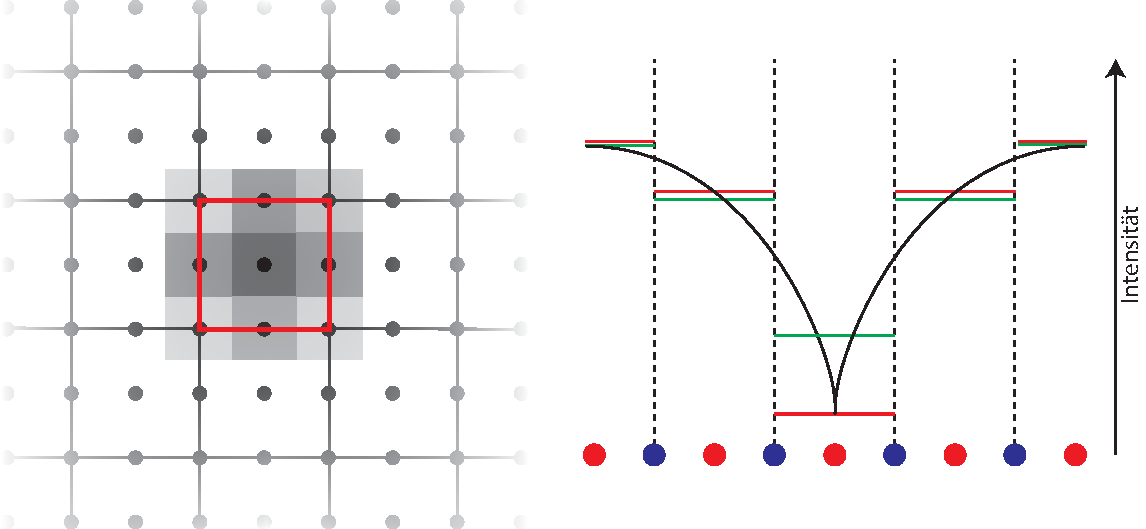
\includegraphics[width=0.9\textwidth]{images/average.pdf}
	\caption[Gewichteter Mittelwert]{Die Verwendung von Überabtastung und gewichteten Mittelwertes bei den Streubildern: Um die Intensität im links rot umrandeten Bereich zu bestimmen, wird die Intensität an den Schwarzen Punkten berechnet und ein gewichteter Mittelwert gebildet, indem die Intensität der vier Randwerte zur Hälfte, die der vier Eckpixel zu einem Viertel in dem umrandeten Bereich mitberücksichtigt werden. Der Effekt gegenüber einer Berechnung nur in den Zentren der Pixel zeigt sich rechts: Wird die Intensität bei einem schwarz dargestellten wahren Intensitätsverlauf nur an den roten Punkten bestimmt, dominiert das Minimum den Intensitätsverlauf. Eine geringere Abweichung ergibt sich bei Berechnung auch an den blauen Punkten und Bildung des gewichteten Mittelwert (grün).}
	\label{fig:average}
\end{figure}%
\clearpage
\section{Ergebnisse Simulation}
\begin{figure}[H] %exitwave und scatter
	\centering
	\begin{subfigure}[b]{0.49\textwidth}
		\setbox1=\hbox{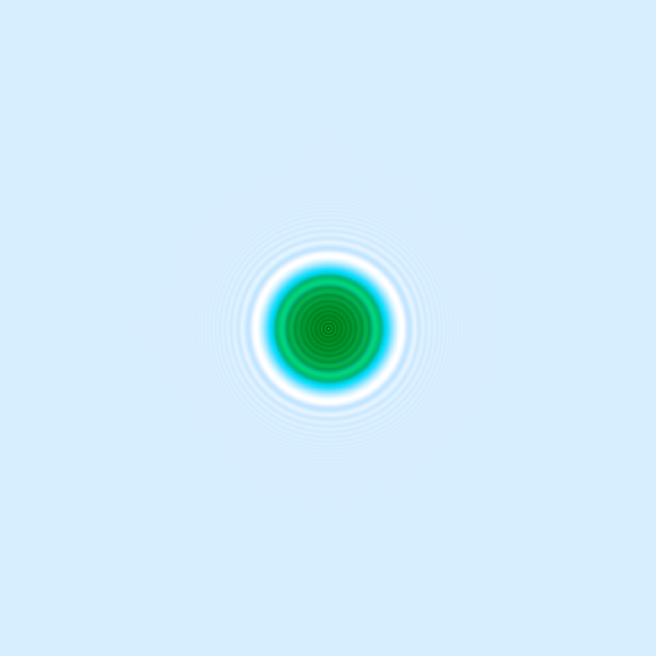
\includegraphics[width=\textwidth]{images/fig_sim_exitwave_multislice-r100-bd1e-3.png}}
		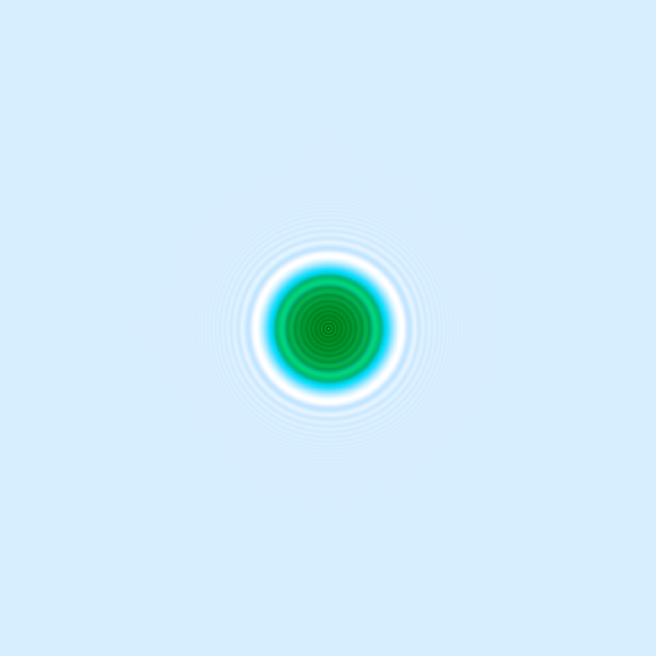
\includegraphics[width=\textwidth]{images/fig_sim_exitwave_multislice-r100-bd1e-3.png}\llap{\makebox[\wd1][l]{\includegraphics[width=0.5\textwidth]{images/fig_sim_exitwave_multislice_cw-r100-bd1e-3.pdf}}}
		\caption{Austrittswelle}
		\label{fig:exitwave}
	\end{subfigure}
	\begin{subfigure}[b]{0.49\textwidth}
		\setbox1=\hbox{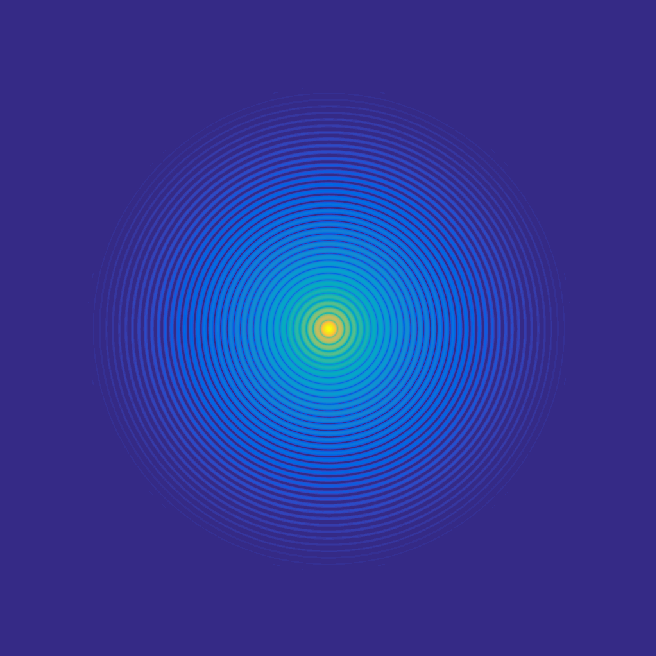
\includegraphics[width=\textwidth]{images/fig_sim_scatter_multislice-r100-bd1e-3.png}}
		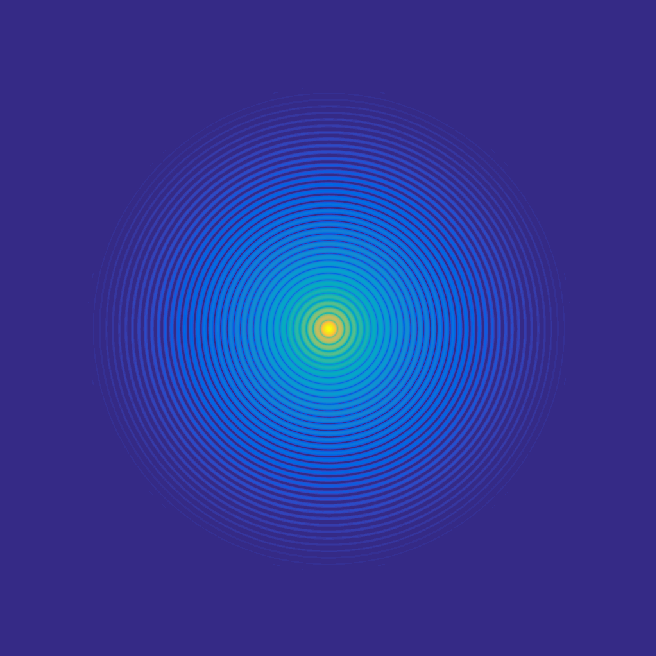
\includegraphics[width=\textwidth]{images/fig_sim_scatter_multislice-r100-bd1e-3.png}\llap{\makebox[\wd1][l]{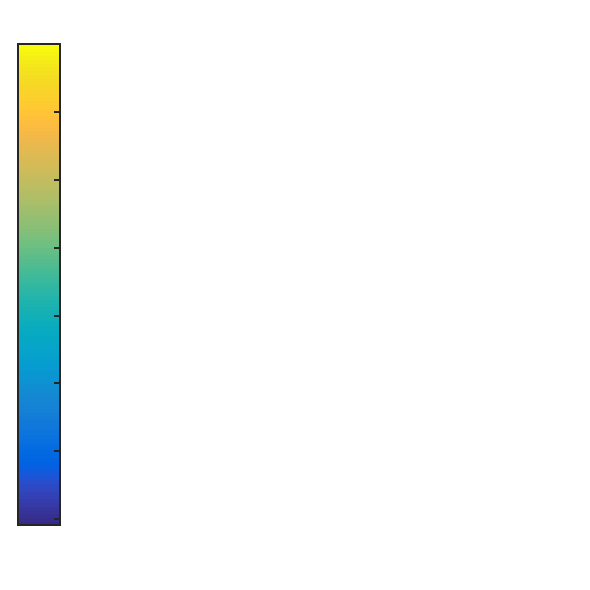
\includegraphics[width=0.5\textwidth]{images/fig_sim_scatter_multislice_cb-r100-bd1e-3.pdf}}}
		\caption{Streubild}
		\label{fig:scatter}
	\end{subfigure}
	\caption[Austrittswelle und Streubild einer Kugel]{Exemplarische Multislice-Propagations Austrittwelle (a) und (logarithmiertes) Streubild (b) einer Kugel mit Radius \SI{100}{nm} bei $\beta,\delta$=$10^{-3}$. Die relative Intensität der Austrittswelle bezüglich der Eintrittswelle ist über die Helligkeit dargestellt, die Phase über den Farbton. Das Streubild zeigt einen Bereich bis 15°.}
	\label{fig:exitscatter}
\end{figure}%
\begin{figure}[H] %rel error
	\centering
	\begin{subfigure}[b]{0.48\textwidth}
		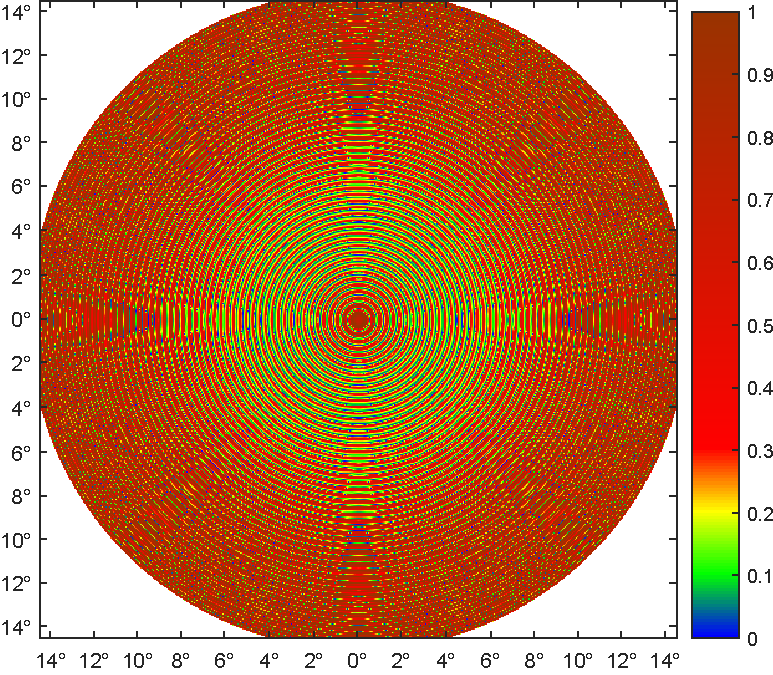
\includegraphics[width=\textwidth]{images/fig_sim_relerror_FTproj-r100-bd1e-3.pdf}
		\caption{Projektion}
	\end{subfigure}\hfill
	\begin{subfigure}[b]{0.48\textwidth}
		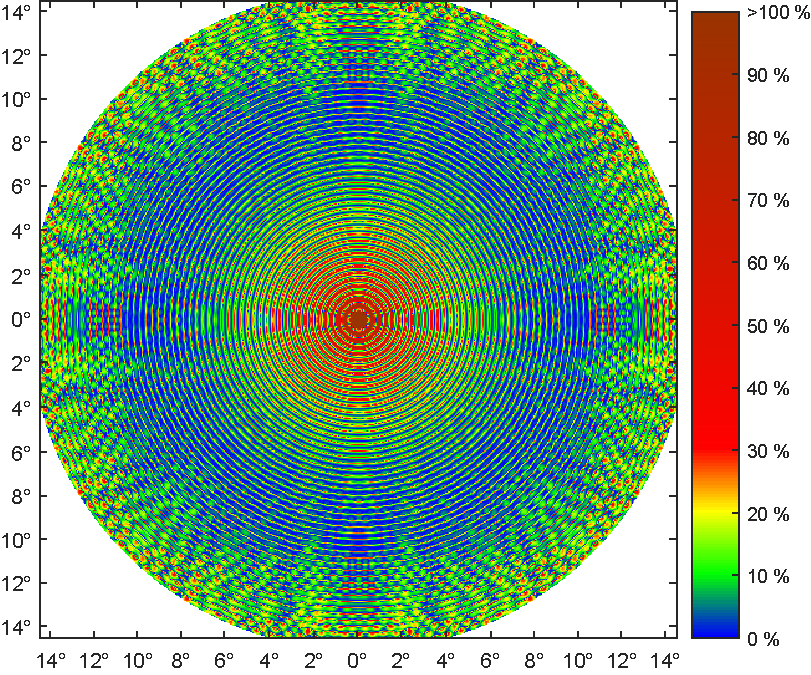
\includegraphics[width=\textwidth]{images/fig_sim_relerror_msft-r100-bd1e-3.pdf}
		\caption{MSFT}
	\end{subfigure}
	\par\bigskip
	\begin{subfigure}[b]{0.48\textwidth}
		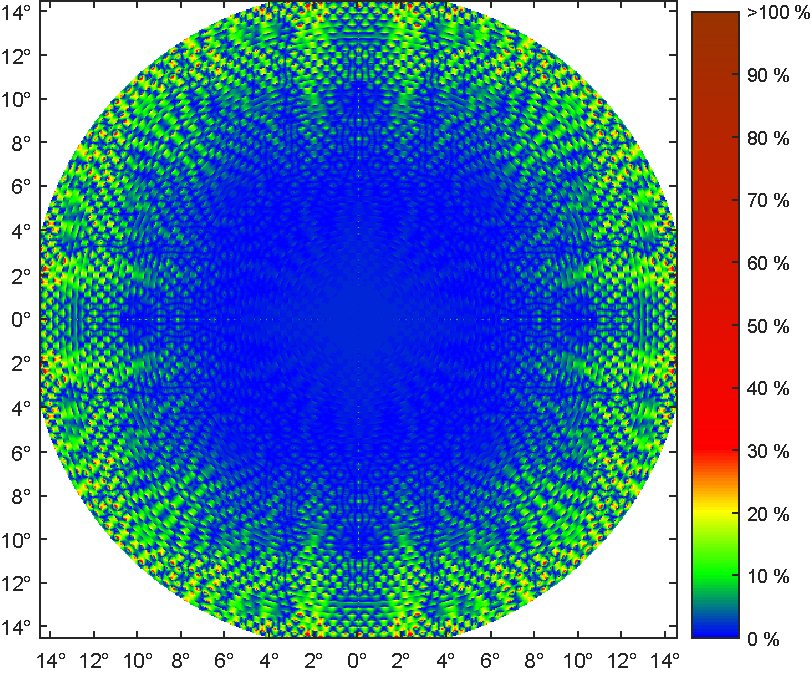
\includegraphics[width=\textwidth]{images/fig_sim_relerror_thibault-r100-bd1e-3.pdf}
		\caption{Thibaults Multislice}
	\end{subfigure}\hfill
	\begin{subfigure}[b]{0.48\textwidth}
		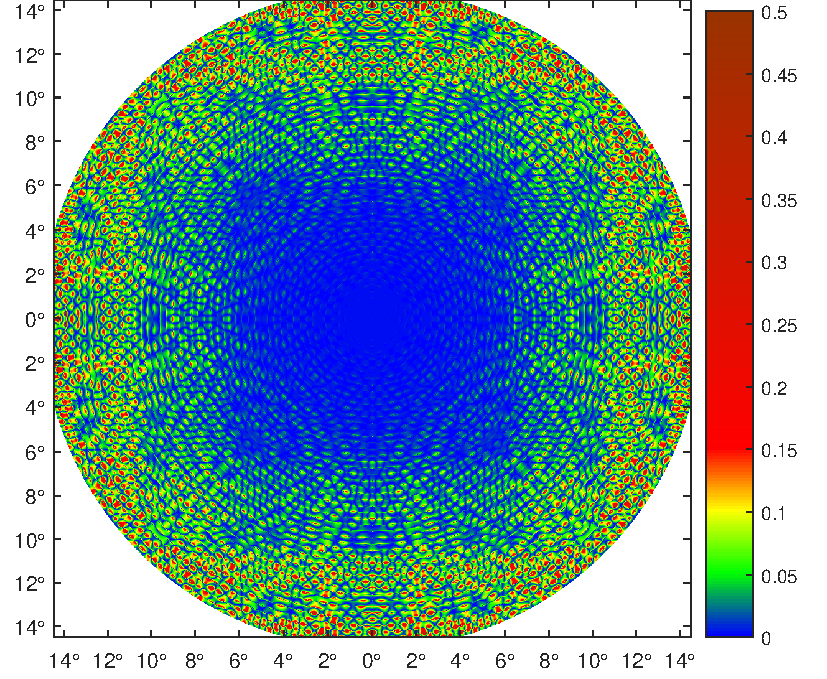
\includegraphics[width=\textwidth]{images/fig_sim_relerror_multislice-r100-bd1e-3.pdf}
		\caption{Multislice Propagation}
	\end{subfigure}
	\caption[Relativer Fehler der Simulationen]{Relative Abweichungen von Mie der simulierten Streubilder einer Kugel mit Radius \SI{100}{nm} bei $\beta=\delta=10^{-3}$. }
	\label{fig:relerror}
\end{figure}
\clearpage
\begin{sidewaysfigure} %profile
	\centering
	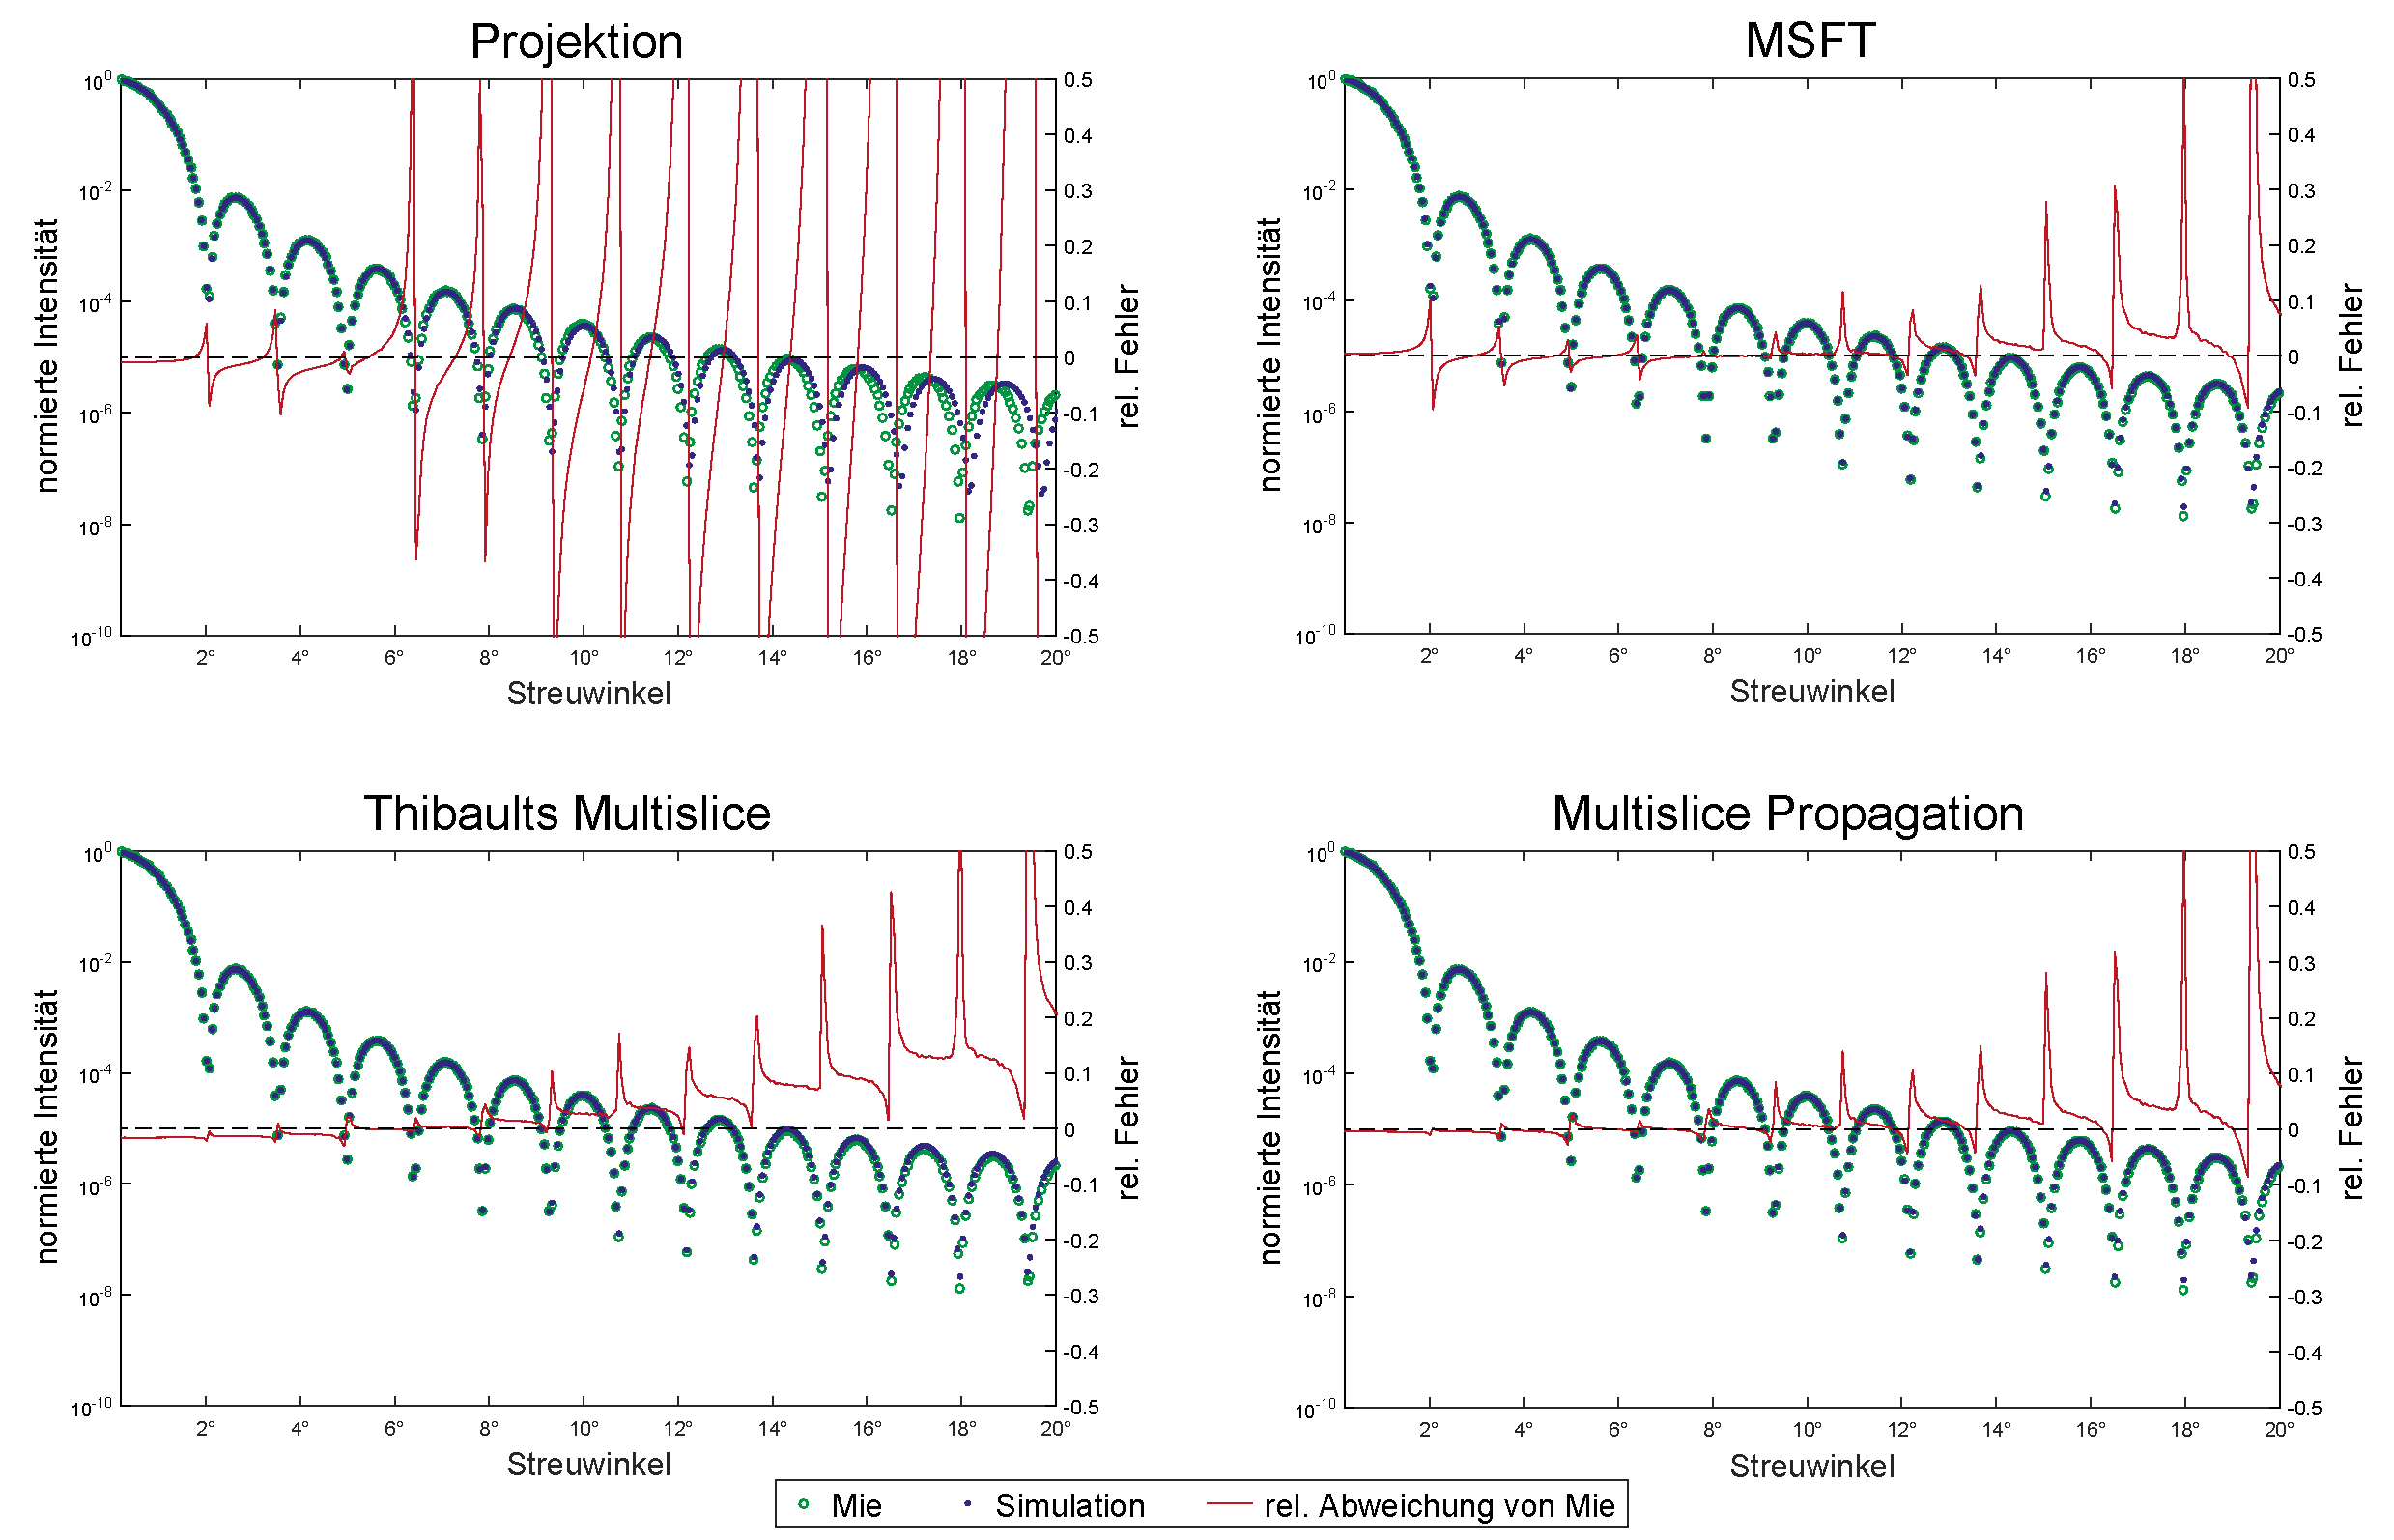
\includegraphics[width=1\textwidth]{images/fig_sim_profile.pdf}
	\caption[Radiale Profile]{Radiale logarithmierte Intensitätsprofile berechnet mit den verschiedenen Algorithmen sowie die relative Abweichung von Mie für eine Kugel mit Radius \SI{20}{nm} und $\beta,\delta$=$10^{-4}$. Es ist bei kleinen Streuwinkeln eine gute Übereinstimmung aller Algorithmen zu erkennen, bei höheren Winkeln versagt die Projektion. Über den gesamten Bereich besitzt bei diesen Parametern die Multislice Propagation die beste Übereinstimmung. Die relativen Fehler der Simulationen sind in den Intensitätsminima aufgrund der dort deutlich abfallenden Referenzintensität bei allen Verfahren deutlicher ausgeprägt.}
	\label{fig:profil}
\end{sidewaysfigure}
\clearpage

\begin{figure}[H] %parameter variation
	\centering
	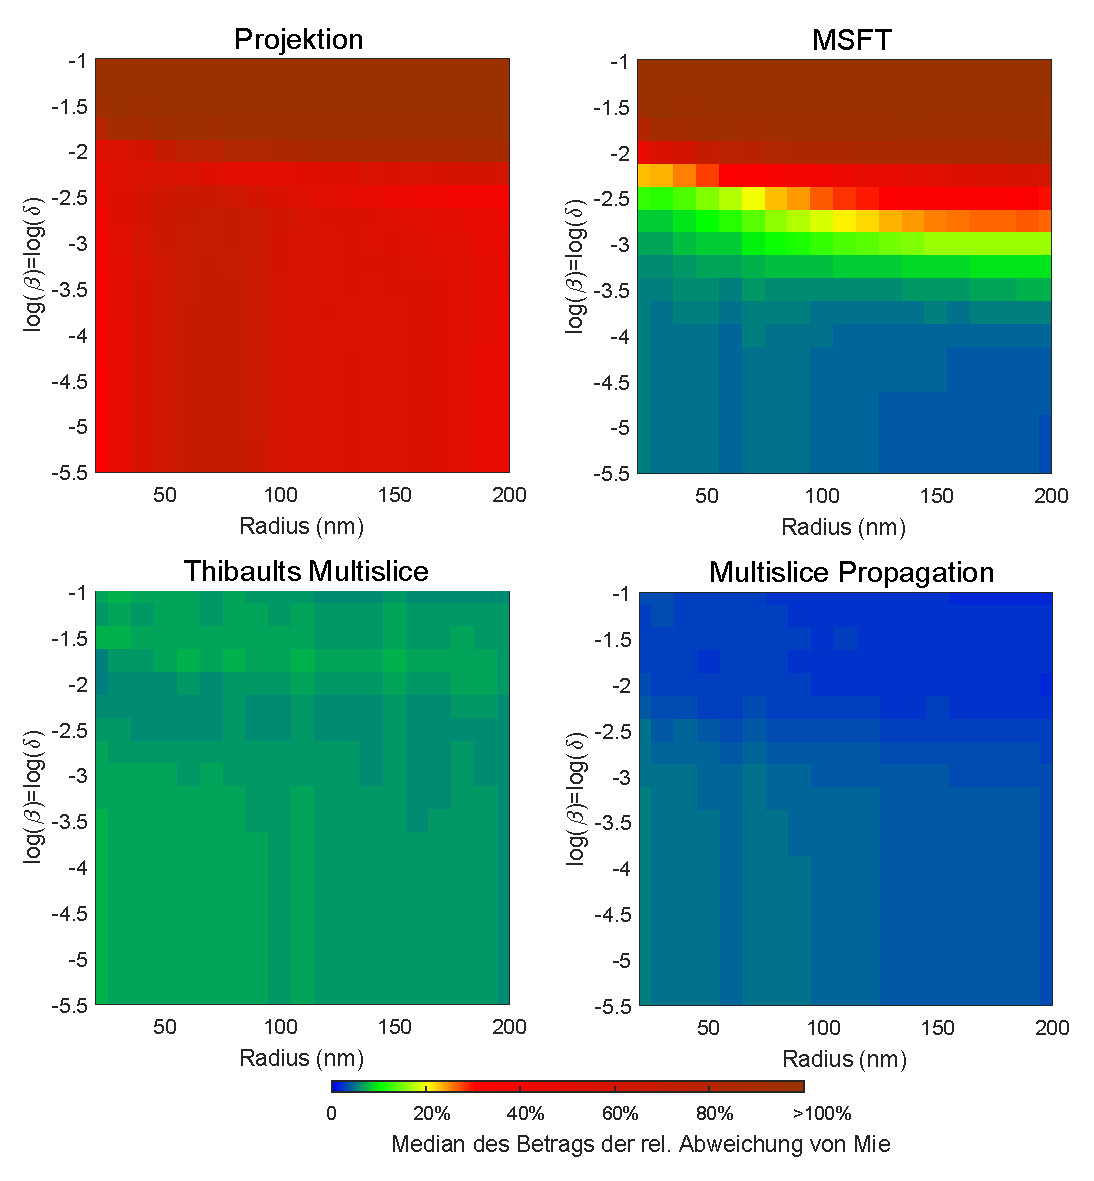
\includegraphics[width=1\textwidth]{images/fig_sim_var.pdf}
	\caption[Gültigkeit der Simulationsalgorithmen]{Zur Entscheidung bei welchen Radien und welchen Abweichung der Brechzahl vom Vakuum die Simulationen noch valide sind, ist die mediane, relative Abweichung bis 20° von Mie über den Parametern aufgetragen. Es somit die Bereiche erkennbar, in denen der jeweilige Simulationsalgorithmus valide Ergebnisse liefert. Parameter: $\Delta x=\sfrac{\lambda}{2}$, $\Delta z$ als $\sfrac{\lambda}{8}$ und N=2048.}
	\label{fig:variation}
\end{figure}

\section{komplexeres Objekt}
\begin{table}[H]
	\begin{minipage}[b]{.64\textwidth }%
	 	\begin{small}
 			\begin{tabular}{lll}
 				\hline
 				Material													&Brechzahl bei \SI{1}{nm}~\cite{henke}\\
 				\hline
 				Lecithin (\chem{C_{44}H_{82}NO_8P})~\cite{milo2015}			&$1-(1.69-0.12i)\times10^{-4}$			\\ 					
 				Wasser														&$1-(1.55-0.18i)\times10^{-4}$			\\
 				Protein (\chem{H_{86}C_{52}N_{13}O_{15}S})~\cite{bergh2008}	&$1-(2.03-0.16i)\times10^{-4}$			\\
 				Xenon-Cluster												&$1-(2.54-1.46i)\times10^{-4}$			\\
 				\hline
 			\end{tabular}
		\end{small}
		\centering
		\caption[Für die Berechnung der komplexen Austrittswelle verwendete Materialien]{Brechzahlen der verwendeten Materialien}   \label{tab:brechzahl}
	\end{minipage}
	\begin{minipage}[b]{.35\textwidth}
				\hspace*{0pt}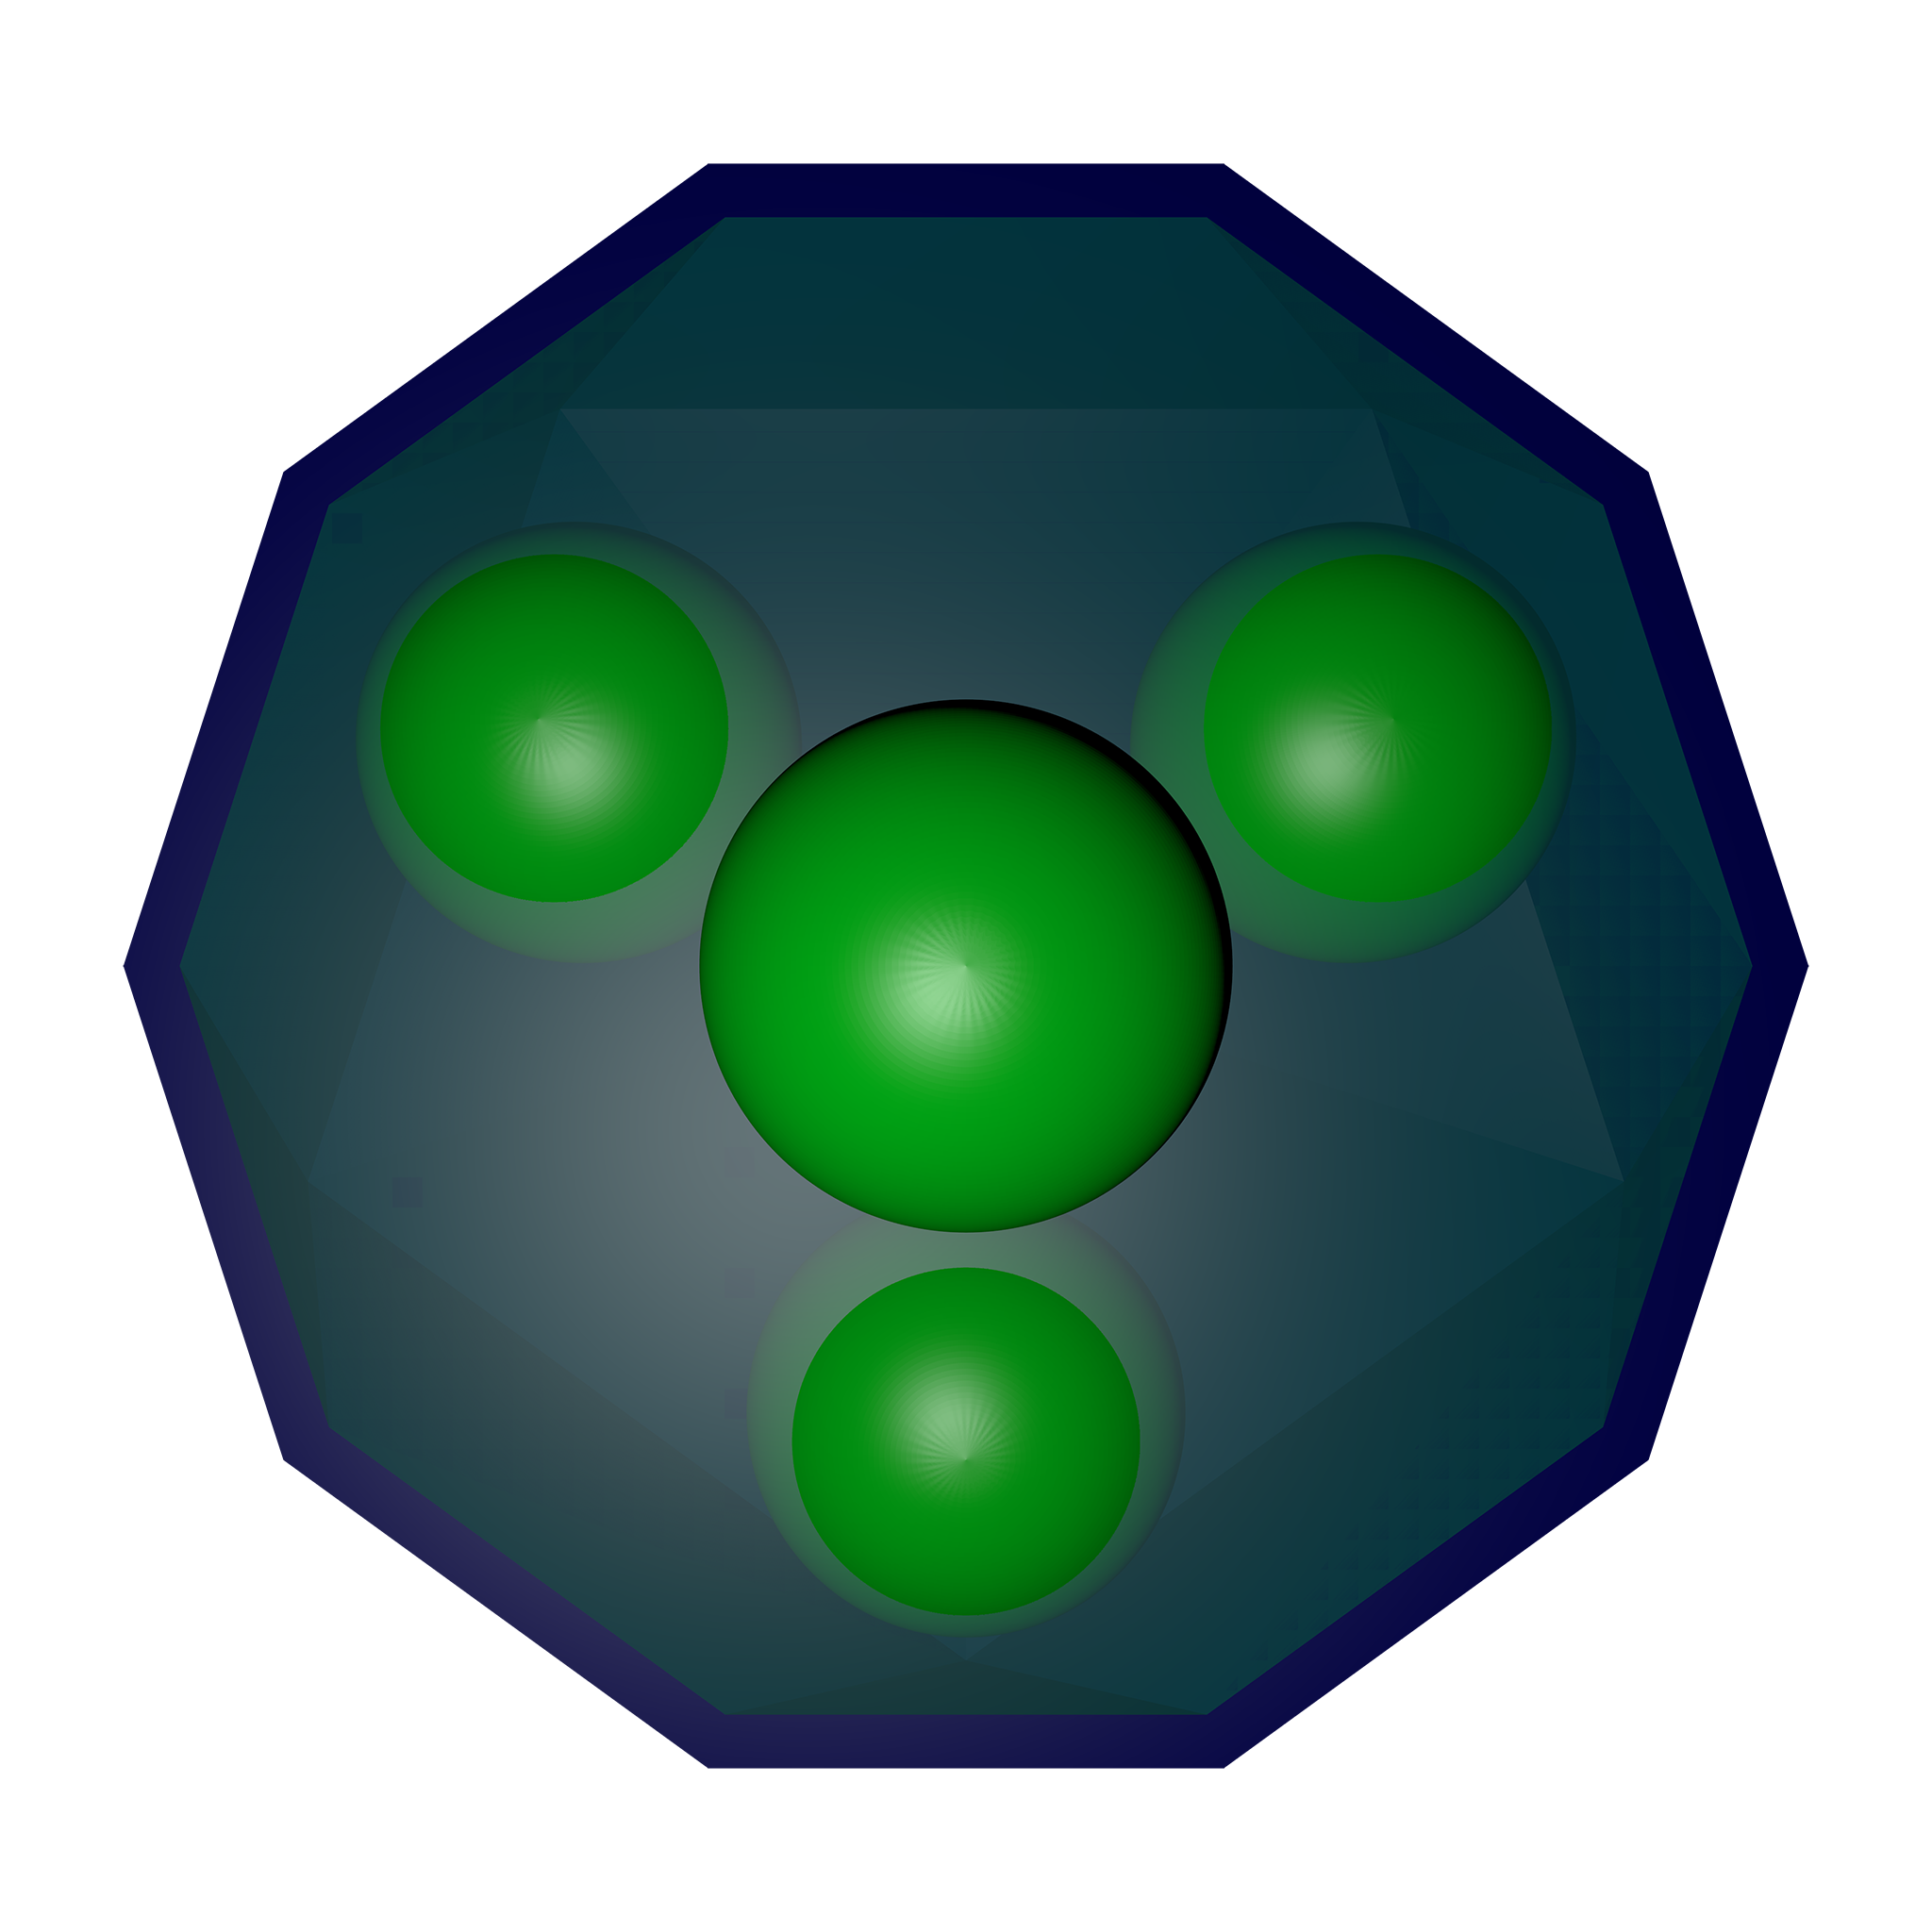
\includegraphics[width=.8\textwidth]{images/scene.png}%
				\captionof{figure}{3D-Modell\label{fig:komplexmodel}}%
	\end{minipage}
	\par\bigskip
\end{table}


\begin{figure}[H] %exitwave und scatter
	\begin{subfigure}[b]{0.49\textwidth}
		\setbox1=\hbox{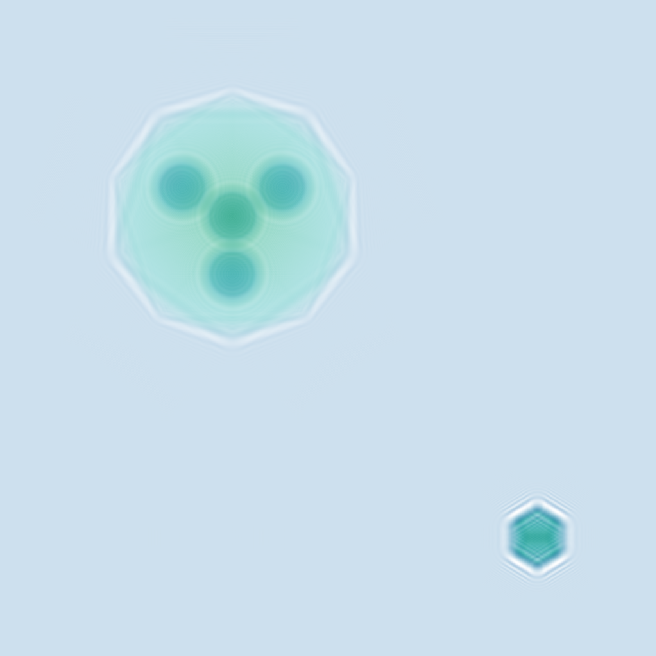
\includegraphics[width=\textwidth]{images/fig_simholo_v2_exitwave.png}}
		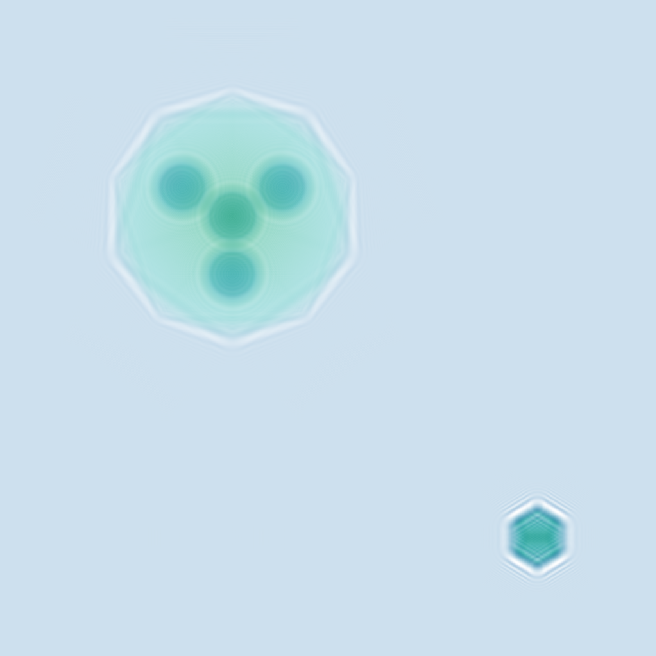
\includegraphics[width=\textwidth]{images/fig_simholo_v2_exitwave.png}\llap{\makebox[\wd1][l]{\includegraphics[width=0.5\textwidth]{images/fig_simholo_v2_exitwave_cw.pdf}}}
		\caption{Austrittswelle}
		\label{fig:komplexexit}
	\end{subfigure}
	\begin{subfigure}[b]{0.49\textwidth}
		\setbox1=\hbox{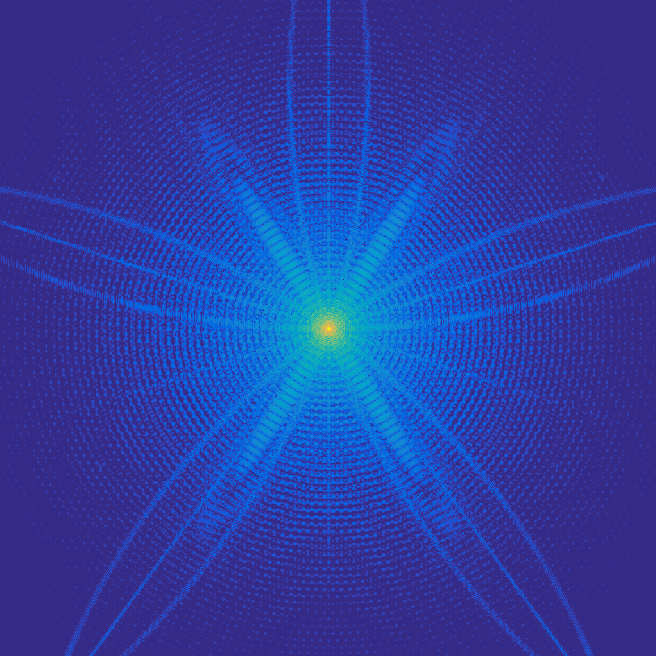
\includegraphics[width=\textwidth]{images/fig_simholo_v2_scatter.png}}
		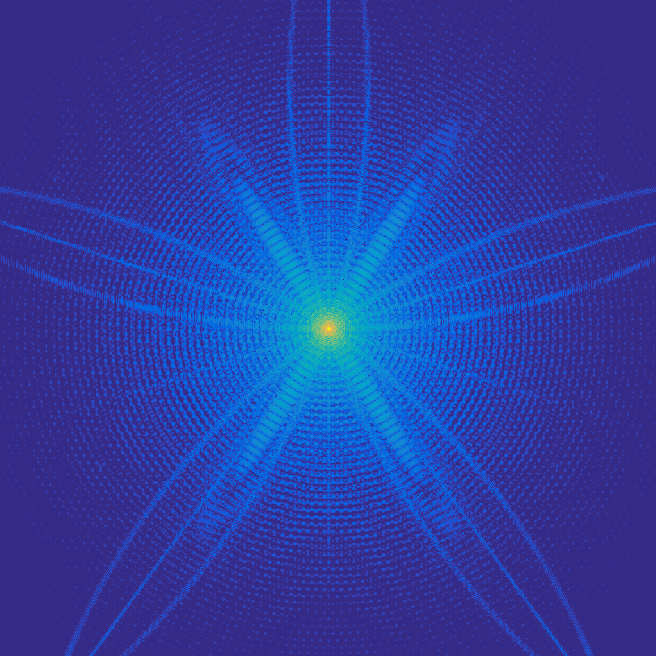
\includegraphics[width=\textwidth]{images/fig_simholo_v2_scatter.png}\llap{\makebox[\wd1][l]{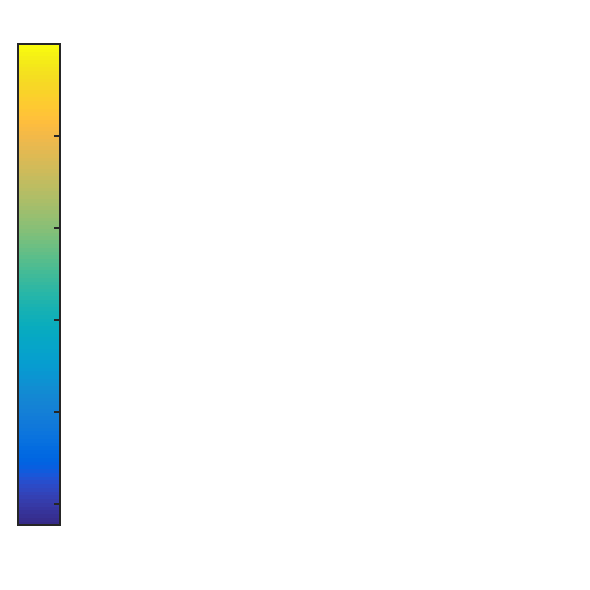
\includegraphics[width=0.5\textwidth]{images/fig_simholo_v2_scatter_cb.pdf}}}
			\caption{Streubild}
			\label{fig:komplexscatter}
	\end{subfigure}		
	\caption[Austrittswelle und Streubild eines komplexen Objektes]{Austrittswelle und logarithmiertes Streubild eines komplexen Objektes. Bei der Austrittswelle ist die relative Intensität bezüglich der Eintrittswelle über die Helligkeit dargestellt, die Phase über den Farbton.}
	\label{fig:komplex}
\end{figure}
\clearpage
\section{Rekonstruktion}
\subsection{Phasenrekonstruktion:Support}
Holographie: Kreuzkorrelation aus Referenz und Objekt als Support. Shrink-Wrap:  Autokorrelation als initialem Support und Anpassung im Laufe der Rekonstruktion.
\begin{figure}[H]
	\centering
	\begin{subfigure}[b]{0.9\textwidth}
		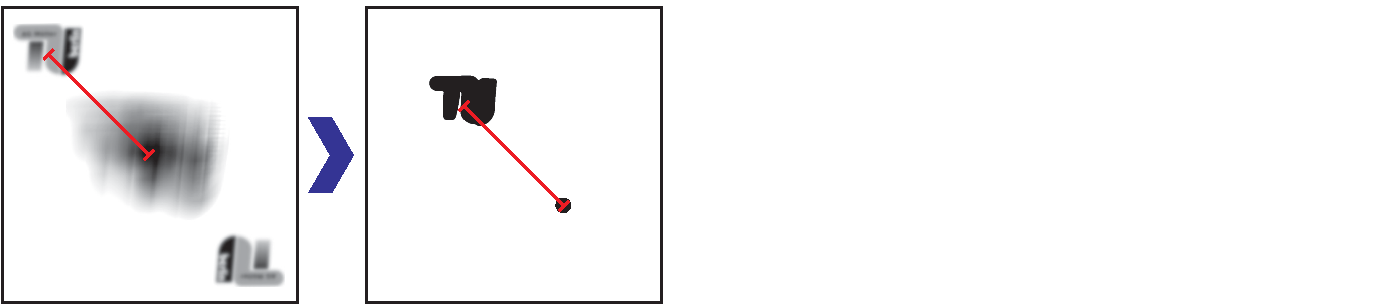
\includegraphics[width=\textwidth]{images/support_holo.pdf}
		\caption{Holographie}
	\end{subfigure}\\

	\begin{subfigure}[b]{0.9\textwidth}
		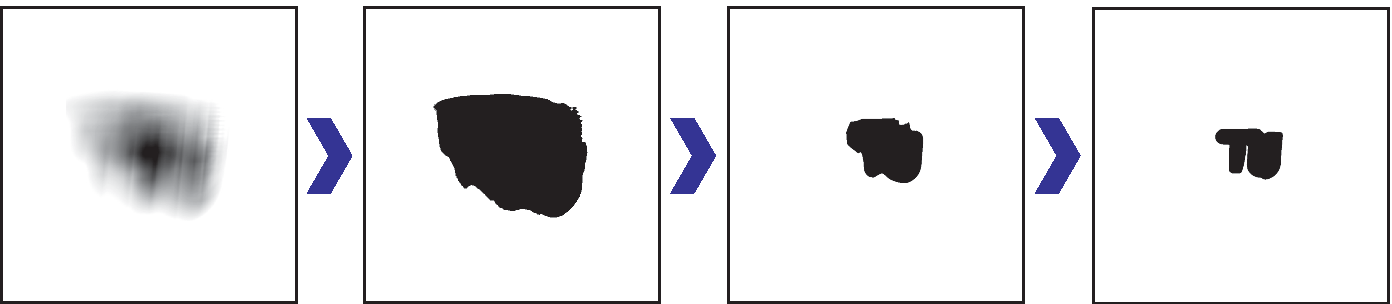
\includegraphics[width=\textwidth]{images/support_sw.pdf}
		\caption{Shrink-Wrap}	
	\end{subfigure}
	
	\label{fig:support}
\end{figure} 

\subsection{Vergleich in 2D}
\paragraph{Ideal}
Rekonstruktion mit Zentralstrahl ohne Rauschen. 
\begin{figure}[H]
	\reconimage{[width=.48\textwidth]{images/recon2d-perfect.png}}
	
	\label{fig:recon2d-perfect}
\end{figure}
\clearpage
\paragraph{Einfluss Zentralmaske}
Einfluss einer zentralen Maskierung des Streubildes mit Radius 16 Pixel bzw. 64 Pixel von 2048 Pixeln
\begin{figure}[H]
	
	\begin{subfigure}[b]{0.48\textwidth}
		\reconimage{[width=\textwidth]{images/recon2d-mask16.png}}
		\caption{kleine Maske}
	\end{subfigure}
	\hspace*{\fill}
	\begin{subfigure}[b]{0.48\textwidth}
		\reconimage{[width=\textwidth]{images/recon2d-mask64.png}}
		\caption{große Maske}	
	\end{subfigure}
	\label{fig:recon2d-mask}
\end{figure}

\paragraph{Einfluss Rauschen}
Einfluss des Rauschen: Das gering maskierte Streubild wurde mit 16\,Bit bzw 14\,Bit diskretisiert und Poisson-Shot-Rauschen hinzugefügt.
\begin{figure}[H]
	\begin{subfigure}[b]{0.45\textwidth}
		\reconimage{[width=\textwidth]{images/recon2d-mask16bit16.png}}
		\caption{wenig Rauschen}
	\end{subfigure}
	\hspace*{\fill}
	\begin{subfigure}[b]{0.45\textwidth}
		\reconimage{[width=\textwidth]{images/recon2d-mask16bit14.png}}
		\caption{viel Rauschen}	
	\end{subfigure}
	\label{fig:recon2d-noise}
\end{figure}
\clearpage
\paragraph{Einfluss Referenzabschätzung}
Das gering verrauschte und maskierte Streubild wird mit einem andren Radius der kreisförmigen Referenz rekonstruiert. Dies hat nur einen Einfluss auf die Entfaltung.
\begin{figure}[H]
	\begin{subfigure}[b]{0.45\textwidth}
		\reconimage{[width=\textwidth]{images/recon2d-mask16bit16error01.png}}
		\caption{1\% Abweichung des Radius}
	\end{subfigure}
	\hspace*{\fill}
	\begin{subfigure}[b]{0.45\textwidth}
		\reconimage{[width=\textwidth]{images/recon2d-mask16bit16error05.png}}
		\caption{5\% Abweichung des Radius}	
	\end{subfigure}

	\label{fig:recon2d-ref}
\end{figure}
\clearpage
\paragraph{Rekonstruktion 3D Austrittswelle}
 Dargestellt ist jeweils das Ergebnis normiert auf das optimale Ergebnis mit der aus \ref{fig:komplex} bekannten Farbskala.
\begin{figure}[H]
	\centering
	\reconimage{[width=.75\textwidth]{images/recon3d-v2.png}}
	\label{fig:recon3d}
\end{figure}	


\end{document}
